\documentclass{article}
\usepackage{tikz}
\usetikzlibrary{shapes.geometric, arrows, positioning, decorations.pathreplacing, calc, matrix, fit}


\begin{document}

\begin{figure}[h!]

\begin{tikzpicture}[node distance=2cm and 2cm,
  inner/.style={circle,draw=blue!50,fill=blue!20,thick,inner sep=3pt},
  outer/.style={draw=green,fill=green!20,thick,inner sep=10pt},
  mymatrix/.style={matrix of nodes, nodes=typetag, row sep=1em},
  mycontainer/.style={draw=gray, inner sep=1ex},
  typetag/.style={draw=gray, inner sep=1ex, anchor=west},
  title/.style={draw=none, color=gray, inner sep=0pt},
  ]

  \node[outer, remember picture] (input) at (-8cm, 0) {
    \begin{tikzpicture}
    \foreach \x in {1,...,4}
    {
      \node[yslant=0.5] (wsi\x) at (\x*.8-4,0) {
        \includegraphics[width=.1\textwidth, height=.1\textheight]{./wsi\x.png}
      };
    }
  % Calculate the coordinates for the box
  \path (wsi1.south west) ++(0,-0.1) coordinate (bottom left);
  \path (wsi4.north east) ++(0,0.1) coordinate (top right);

  % Draw the box around the images
  \draw[black, thick] (bottom left) rectangle (top right);
  \node[below=0.0cm of bottom left, anchor=north west, text width=4.2cm, align=center] (label) {Training Data};

  \matrix[mymatrix, below=0.1cm of label, draw] (mx1) {
    |[title]| \\
    Labels \\
    Sensitive Variables \\
  };
  \node[below=0.0cm of mx1, text width=4.2cm, align=center] (label) {Annotations};
Annotations

  \end{tikzpicture}
};


\coordinate [right=3cm of input] (Model) {};
  \node[outer, remember picture] (training) at (Model) {
    \begin{tikzpicture}
\def\numLayers{5}
\def\offset{0.2}
\foreach \n in {1,...,\numLayers}
{
    \pgfmathsetmacro{\shiftX}{(\numLayers - \n) * \offset}
    \pgfmathsetmacro{\shiftY}{(\numLayers - \n) * \offset / 2}

    \draw[fill=blue!30, opacity=0.9] ([shift={(\shiftX, \shiftY)}]Model) rectangle ++(.4,-2);
}

      \node at ([shift={(2*\offset, -\numLayers*\offset - 1.5)}]Model) (ssl) {SSL Model};


\node[below left=-.2cm and .-3cm of ssl] (monai) {
  
\includegraphics[width=.1\textwidth, height=.1\textheight]{./MONAI-logo-color.png}
};

\node[below right=0.1cm and .-3cm of ssl] (pytorch) {
  
\includegraphics[width=.1\textwidth, height=.1\textheight]{./Pytorch_logo.png}
};

\end{tikzpicture}
  };

\node[outer, remember picture, right=3cm of Model] (output) {
    \begin{tikzpicture}

      \node[yslant=0.5] (wsiMap) {
        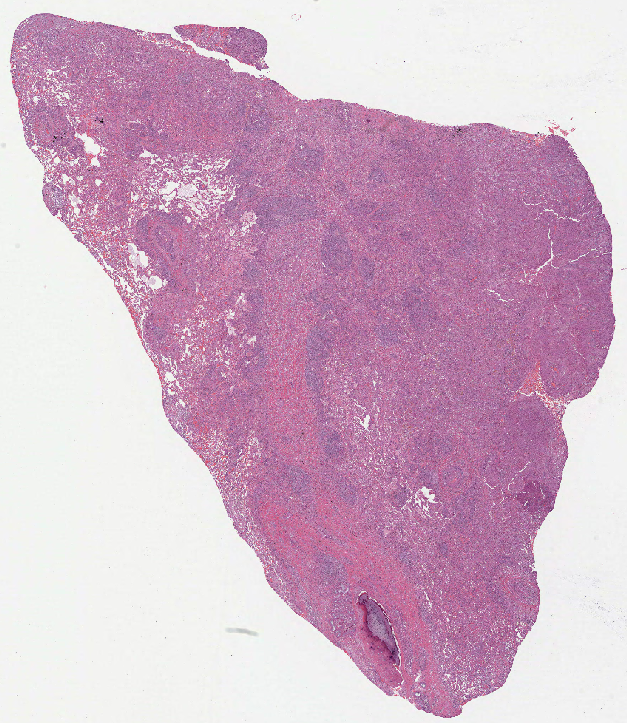
\includegraphics[width=.1\textwidth, height=.1\textheight]{./wsi1.png}
      };

      \node[right=of wsiMap] (mapper) {
        \begin{tikzpicture}
\foreach \y in {0,1,...,8}
    {
        \node[circle, draw=black, fill=green, minimum size=0.01cm, scale=.3] at (0, -\y*0.7) {};
    }
          \end{tikzpicture}
        };

      \draw[->] (wsiMap) edge ([shift={(0cm,-.45cm)}]mapper.west);

      \node [below=.0cm of mapper] (ssl) {Feature vector};

    \end{tikzpicture}
  };

\node [above=.0cm of input] (inputText) {Input};
\node [above=.0cm of training] (trainingText) {Training};
\node [above=.0cm of output] (outputText) {Output model};


 
 
\end{tikzpicture}
\end{figure}

\end{document}

